

\section{Model including the second fish}

\begin{flushleft}
    The fishowner desperately wanted two types of competing fish species:
    rainbowfish and gourami.
    To make sure that both fishes both had enough food and didn't manage to kill eachother
    we made a system of differential equations. In this case they interact with each other.
    There is a 4\% chance that a gourami will kill a rainbowfish, thus the $-0.04PG$.
\end{flushleft}

\begin{align*}[left = \empheqlbrace]
    \frac{dP}{dt}= 0.7P-0.007P^2-0.04PG \\
    \frac{dG}{dt} = -0.25G+0.008PG
\end{align*}

\begin{flushleft}
    Now doing the rest was easy. So easy in fact that I wanted to shoot my foot
    with a rocket launcher. The result was the following:

\end{flushleft}
\begin{center}
    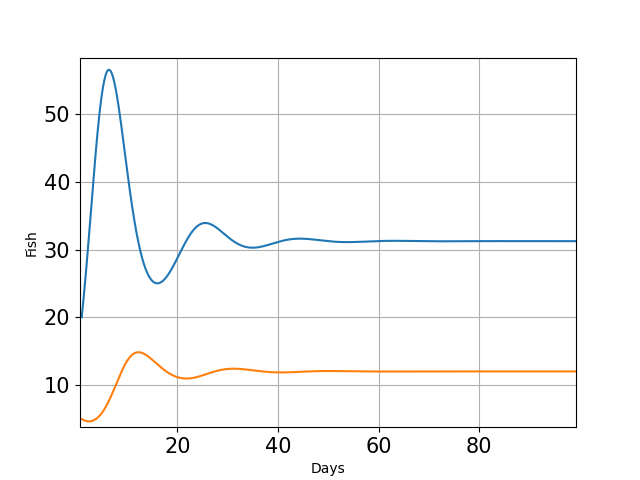
\includegraphics[scale=0.4]{../figures/Figure_2.png}
\end{center}


\begin{equation}
    x
    %\begin{align*}
    % \\ x
    %\end{align*}
    %
\end{equation}